\documentclass[tikz, margin=3mm]{standalone}
\usepackage{tikz}
\usepackage{amsmath}
\usepackage{comment}
\usetikzlibrary{shapes.geometric, arrows, positioning}
\tikzstyle{arrow} = [thick,->,>=stealth]

% flow chart of simulation (zoomed out view)
% uses relative positioning

% Terminal
\tikzstyle{terminal} = [rectangle, rounded corners, minimum width=6cm, minimum height=1cm,text centered, text width=5.5cm, draw=black]

% Process
\tikzstyle{process} = [rectangle, minimum width=6cm, minimum height=1cm, text centered,text width=5.5cm, draw=black]

% Decision
\tikzstyle{decision} = [diamond, aspect=1.8, minimum width=2cm, minimum height=1cm, text centered, text width=2cm, draw=black]

% Subprocess
\newcommand\ppbb{path picture bounding box}
\tikzset{
	subprocess/.style = {rectangle, draw=black, 
		minimum width=6cm, minimum height=1cm, inner xsep=3mm,
		text width =\pgfkeysvalueof{/pgf/minimum width}-2*\pgfkeysvalueof{/pgf/inner xsep},
		align=flush center,
		path picture={\draw 
			([xshift =2mm] \ppbb.north west) -- ([xshift= 2mm] \ppbb.south west)
			([xshift=-2mm] \ppbb.north east) -- ([xshift=-2mm] \ppbb.south east);
		},% end of path picture
	}
}

\tikzstyle{note} = [fill, ellipse,fill=gray!20, node distance=4cm, minimum height=1em, text width=3cm, text centered]

\begin{document}
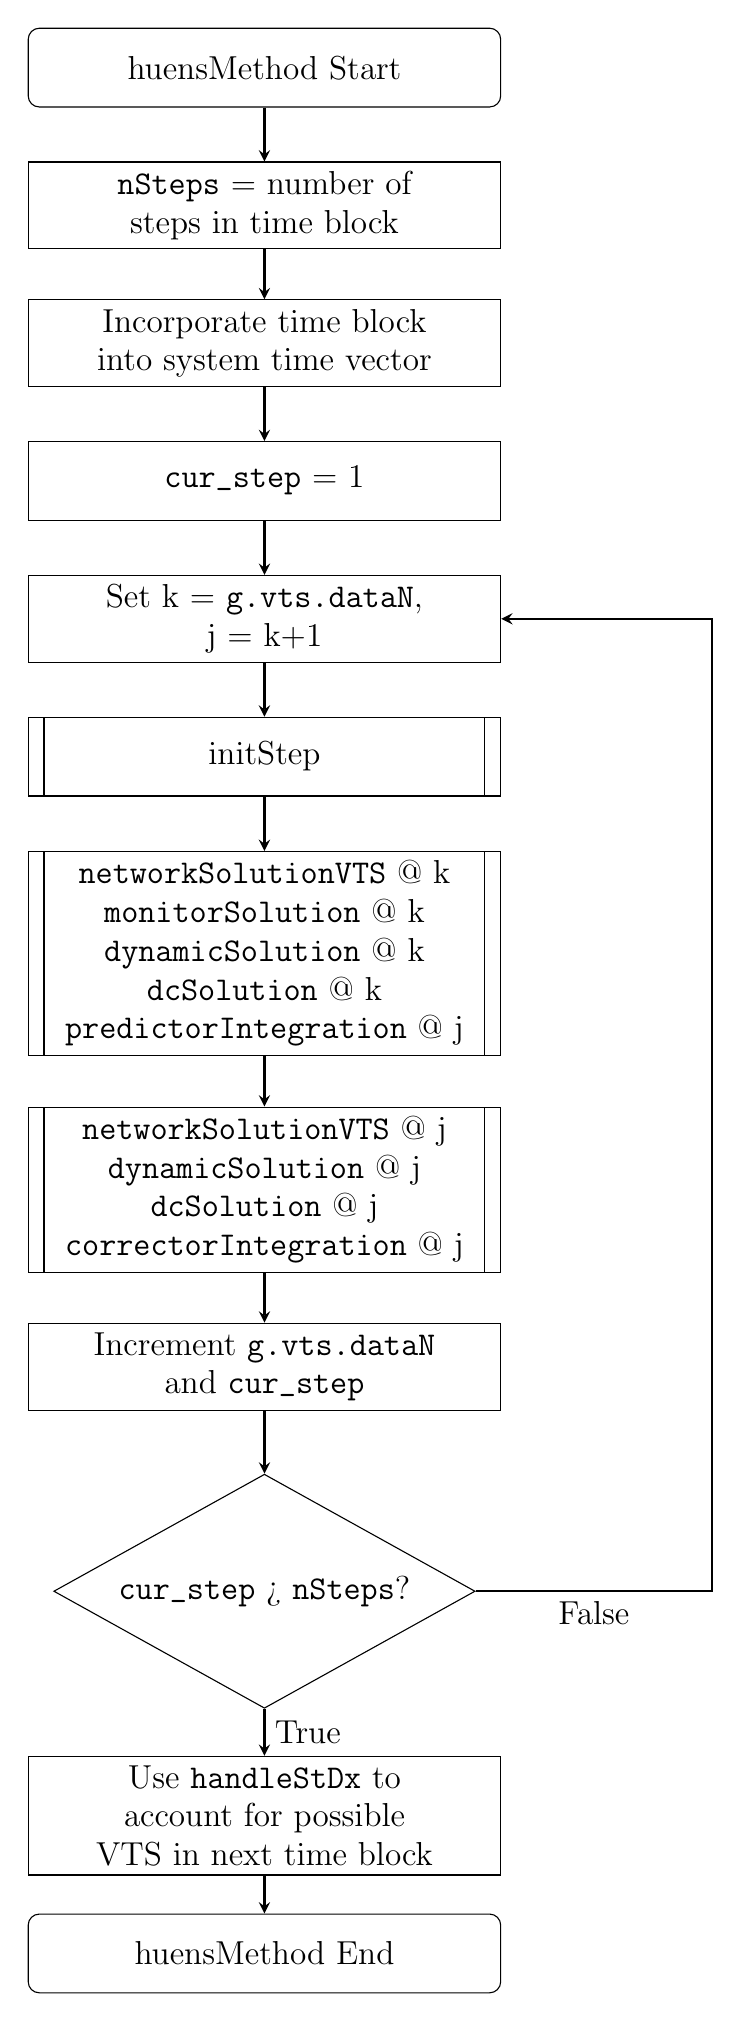
\begin{tikzpicture}[node distance=1.75cm, font=\large] 
% Placement of flowcart nodes
\node (start) [terminal] {huensMethod Start};
\node (getSteps) [process, below of = start] {\verb|nSteps| = number of steps in time block};
\node (incTvec) [process, below of = getSteps] {Incorporate time block into system time vector};
\node (initCstep) [process, below of = incTvec] { \verb|cur_step| = 1};

\node (setLocalIndex) [process, below of = initCstep] {Set k = \verb|g.vts.dataN|, j = k+1};

\node (initStep) [subprocess, below of = setLocalIndex] {initStep};

\node (predictor) [subprocess, below of = initStep, yshift=-.75cm] {{\verb|networkSolutionVTS| @ k \\ \verb|monitorSolution| @ k \\ \verb|dynamicSolution| @ k \\ \verb|dcSolution| @ k \\ \verb|predictorIntegration| @ j}};

\node (corrector) [subprocess, below of = predictor, yshift=-1.25cm] {{\verb|networkSolutionVTS| @ j \\ \verb|dynamicSolution| @ j \\ \verb|dcSolution| @ j \\ \verb|correctorIntegration| @ j}};

\node (incIndices) [process, below of = corrector, yshift=-.5cm] {Increment \verb|g.vts.dataN| and \verb|cur_step|};

\node (checkStep) [decision, below of=incIndices, text width=4cm, yshift=-1.1cm] {\verb|cur_step| > \verb|nSteps|?};

\node (wrapUp) [process, below of = checkStep, yshift=-1.1cm] {Use \verb|handleStDx| to \\account for possible VTS in next time block};

\node (end) [terminal, below of = wrapUp] {huensMethod End};

% Drawing of Lines of main chart
\draw [arrow] (start) -- (getSteps);
\draw [arrow] (getSteps) -- (incTvec);
\draw [arrow] (incTvec) -- (initCstep);
\draw [arrow] (initCstep) -- (setLocalIndex);
\draw [arrow] (setLocalIndex) -- (initStep);
\draw [arrow] (initStep) -- (predictor);
\draw [arrow] (predictor) -- (corrector);
\draw [arrow] (corrector) -- (incIndices);
\draw [arrow] (incIndices) -- (checkStep);
\draw [arrow] (wrapUp) -- (end);

% Draw Decision Lines
%\draw [arrow] (checkStep.east) --  node[anchor=south] {False} (setLocalIndex);
\draw [arrow] (checkStep) --  node[anchor=west] {True} (wrapUp);
\draw [arrow] (checkStep.east) -- node[anchor=north, midway] {False} +(3,0) |- (setLocalIndex);

%% Note nodes AND edges
%\node [left of= start, node distance = 7 cm](title){{\Large }};

%\node [note, right of=start, node distance =5cm](note1){Assumes Data file is provided};
%\draw [arrow,dotted] (note1) -- (start);


\end{tikzpicture}


\end{document}
